\chapter{Geometry and basic facts}

\section{Platonic and Archimedean solids}

Platonic solids are regular \textbf{convex} polyhedra. A regular polyhedron is a polyhedron whose faces are all congruent to a single regular polygon, i.e. a polygon with all sides of equal length. There are exactly five Platonic solids: the tetrahedron, cube, octahedron, dodecahedron, and icosahedron.

Note that convexity is an important property for us, since it ensures that we can always obtain a 3-vertex connected planar graph. This fact is also known as Steinitz’s theorem for polyhedra \cite{kendall24}.

The Archimedean solids can then be obtained by performing one of the following non-disjoint operations on Platonic solids:

\begin{description}
    \item[Truncation] Removes the corners of the polyhedron by making cuts perpendicular to lines connecting the vertices to the centroid of the polyhedron.
    \item[Rectification] A special case of truncation, where the cuts are made in such a way that they pass through the midpoints of the edges connecting the vertices.
    \begin{figure}[H]
        \centering
        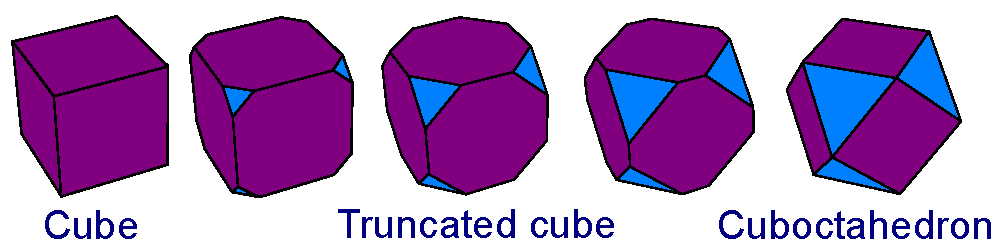
\includegraphics[width=1\textwidth]{../Resources/Figs/op_truncation.pdf}
        \caption{Truncation and rectification of cube visualized \cite{wikimedia-cube-truncation}}
        \label{fig:op_truncation}
    \end{figure}
    \item[Expansion/Cantellation] All facets are moved outward from the centroid of the polyhedron by the same distance, without rescaling. The resulting gaps are filled with regular polygons as follows: edges that were identical in the original polyhedron are connected by inserting a new square, and all vertices that correspond to a single vertex $v$ in the original polyhedron are connected by adding a $d$-gon, where $d = \deg(v)$.

    This operation can also be described as cantellation. The difference is in how we imagine the process that leads to the resulting shape. From the viewpoint of cantellation, we first bevel (cut off) the edges and then apply truncation to what remained from the original vertices.
    \begin{figure}[H]
        \centering
        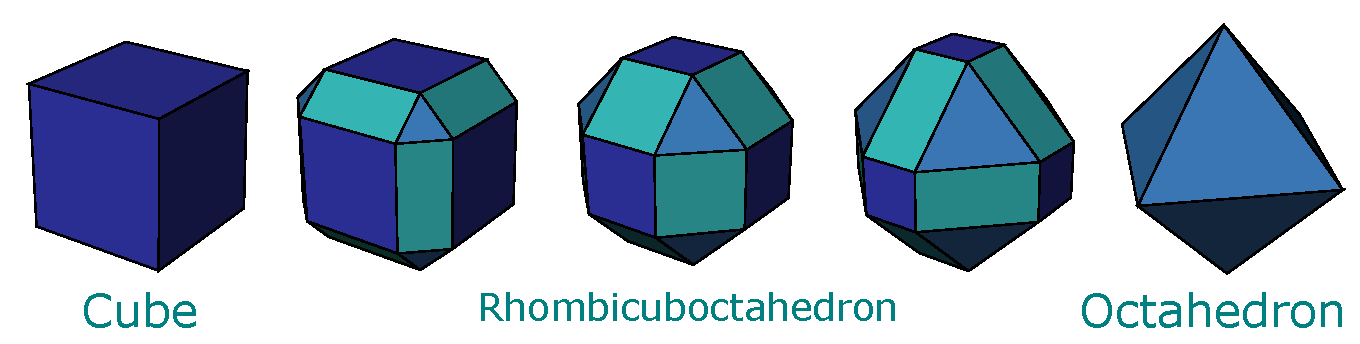
\includegraphics[width=1\textwidth]{../Resources/Figs/op_cantellation.pdf}
        \caption{Cube cantellation visualized \cite{wikimedia-cube-cantellation}}
        \label{fig:op_cantellation}
    \end{figure}
    \item[Snub] Is an application of expansion/cantellation followed by splitting each new square in half in such a way, that we can twist the facets of the original Platonic solid.
    

\begin{figure}[H]
    \centering
    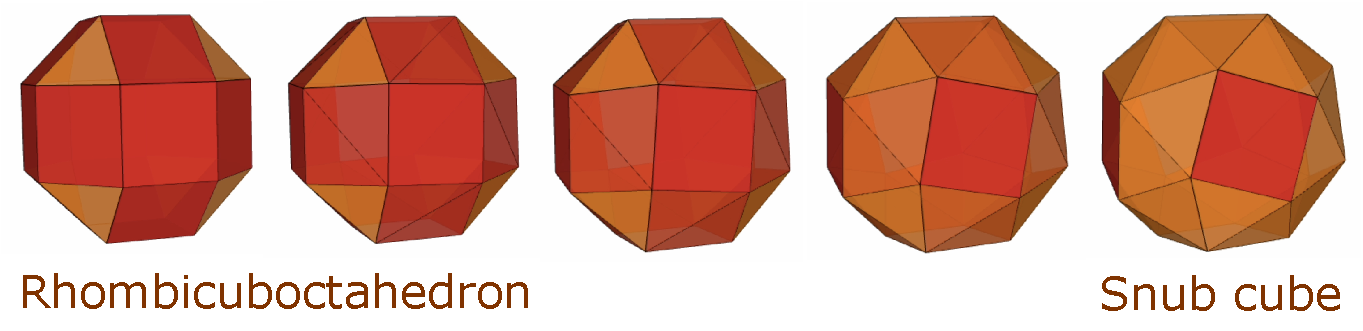
\includegraphics[width=1\textwidth]{Resources/Figs/op_snub_pdfa.pdf}
    \caption{The twisting part of the snub operation on cube visualized \cite{natal-polyhed-viewer}}
    \label{fig:op_snub}
\end{figure}
    
\end{description}

\section{Basic definitions and assumptions}

Here we state mathematical definitions that should not be surprising in any way (i.e. can be considered standard). Also, we state any assumptions we will make, which will then hold for the rest of this thesis.

\begin{defn}[undirected graph]
    An \emph{undirected graph} $G$ is an ordered pair $G = (V,E)$, where $V$ is the set of its vertices and $E \subseteq \binom{V}{2}$ is the set of its edges. 
\end{defn}

Since we are interested in Platonic and Archimedean solids, whose graphs are all planar, it is useful to define the notion of a \textit{plane graph}. This corresponds to a drawing of a graph in the plane with a key property: the edges, as they are drawn, do not cross.

We use the definition of a \textit{drawing} of a graph from the book \textit{Invitation to Discrete Mathematics} by J. Nešetřil and J. Matoušek \cite{matousek2009}. A drawing of a graph may divide the plane into several disjoint, connected regions, which we call the \textit{faces} of the drawing of the graph $G$.

\begin{defn}[planar graph]
    A graph $G$ is \emph{planar} if there exists a drawing of $G$ in the plane without edge crossings.
\end{defn}

\begin{defn}[plane graph]
    A \emph{plane graph} $G' = (V, E, F)$ is a drawing of a planar graph $G = (V, E)$ in the plane, where $F$ is the set of all the faces of the drawing. We will also use the notation $V(G'), E(G'), F(G')$ to refer to the sets $V, E$ and $F$, respectively.
\end{defn}

In this thesis, we assume that for any plane graph $G = (V, E, F)$, the sets $V$, $E$, and $F$ are pairwise disjoint.

\section{Platonic and Archimedean graph properties}

Here we list some properties of the graphs corresponding to the solids described above. Let $G = (V, E, F)$ be a plane graph of a solid, where $F$ is the set of its faces. In the following tables, $d$ denotes a number such that $\forall u \in V : \deg(u) = d$.

The last column shows the so-called \textit{vertex configuration}, which specifies, for each polygon surrounding a vertex, the number of its sides. The numbers appear in the configuration in the exact order in which the corresponding faces are arranged around the vertex. For example, the configuration $c_1 = 3.4.3.4$ differs from the hypothetical configuration $c_2 = 3.4.4.3$, although both contain the numbers $3$ and $4$ exactly twice. In $c_1$, each triangle is surrounded by two squares and vice versa. In $c_2$, each triangle or square has both a triangle and a square next to it.

\begin{table}[H]
\centering
\begin{tabular}{l@{\hspace{1.5cm}}ccccc}
\toprule
\textbf{Platonic} & \textbf{$|V|$} & \textbf{$|E|$} & \textbf{$|F|$} & \textbf{$d$} & \textbf{Vertex config.} \\
\midrule
tetrahedron & 4 & 6 & 4 & 3 & 3.3.3 \\
octahedron & 6 & 12 & 8 & 4 & 3.3.3.3 \\
cube & 8 & 12 & 6 & 3 & 4.4.4 \\
icosahedron & 12 & 30 & 20 & 5 & 3.3.3.3.3 \\
dodecahedron & 20 & 30 & 12 & 3 & 5.5.5 \\
\bottomrule
\end{tabular}
\caption{Basic properties of Platonic graphs}
\label{tab:platonic-basic-props}
\end{table}

\begin{table}[H]
\centering
\begin{tabular}{l@{\hspace{1.5cm}}ccccc}
\toprule
\textbf{Archimedean} & \textbf{$|V|$} & \textbf{$|E|$} & \textbf{$|F|$} & \textbf{$d$} & \textbf{Vertex config.} \\
\midrule
truncated tetrahedron & 12 & 18 & 8 & 3 & 3.6.6 \\
cuboctahedron & 12 & 24 & 14 & 4 & 3.4.3.4 \\
truncated cube & 24 & 36 & 14 & 3 & 3.8.8 \\
truncated octahedron & 24 & 36 & 14 & 3 & 4.6.6 \\
rhombicuboctahedron & 24 & 48 & 26 & 4 & 3.4.4.4 \\
snub cube & 24 & 60 & 38 & 5 & 3.3.3.3.4 \\
icosidodecahedron & 30 & 60 & 32 & 4 & 3.5.3.5 \\
truncated cuboctahedron & 48 & 72 & 26 & 3 & 4.6.8 \\
truncated icosahedron & 60 & 90 & 32 & 3 & 5.6.6 \\
truncated dodecahedron & 60 & 90 & 32 & 3 & 3.10.10 \\
rhombicosidodecahedron & 60 & 120 & 62 & 4 & 3.4.5.4 \\
snub dodecahedron & 60 & 150 & 92 & 5 & 3.3.3.3.5 \\
truncated icosidodecahedron & 120 & 180 & 62 & 3 & 4.6.10 \\
\bottomrule
\end{tabular}
\caption{Basic properties of Archimedean graphs}
\label{tab:archimedean-basic-props}
\end{table}